\section{Part 2: Examination of the Real Data NewData1}

\begin{taskbox}[Part 2: introduction in the lab manual]
The folder of this experiment (\texttt{Lab2\_2}) contains four \texttt{.mat} files with EEG signals (\texttt{NewData1} to \texttt{NewData4}). The signals belong to epileptic patients and were recorded in seizure or non-seizure periods (sampling frequency 250~Hz). The goal is to remove the noise and artifacts of the given signals using the ICA method. Choose two of the four signals and carry out the following steps for each of them.
\end{taskbox}

\subsection*{Questions 1 and 2: Observation and identification of the artifact pattern}
\begin{taskbox}
\textbf{1.} Plot the signal in the time domain, labeling all channels.\\
\textbf{2.} Examine the signal for noise and artifacts. What type of artifact do you see in the signal? In your opinion, can this artifact be removed using the ICA method?
\end{taskbox}

The NewData1 recording consists of 21 channels and the interval from zero to five seconds. Figure~\ref{fig:nd1} shows the original data and the reconstruction with identical vertical spacing and axis range. In some channels a relatively continuous fast oscillation is seen. In the ICA decomposition, component 4 has an oscillatory time course and a narrow peak at 60.059~Hz; about 75.1 percent of its power in 0.5--100~Hz lies in the band 59 to 61~Hz. This evidence is consistent with narrow-band interference near 60~Hz. The exact origin of the equipment or the recording location is not determined from this data alone.

\begin{figure}[H]
\centering
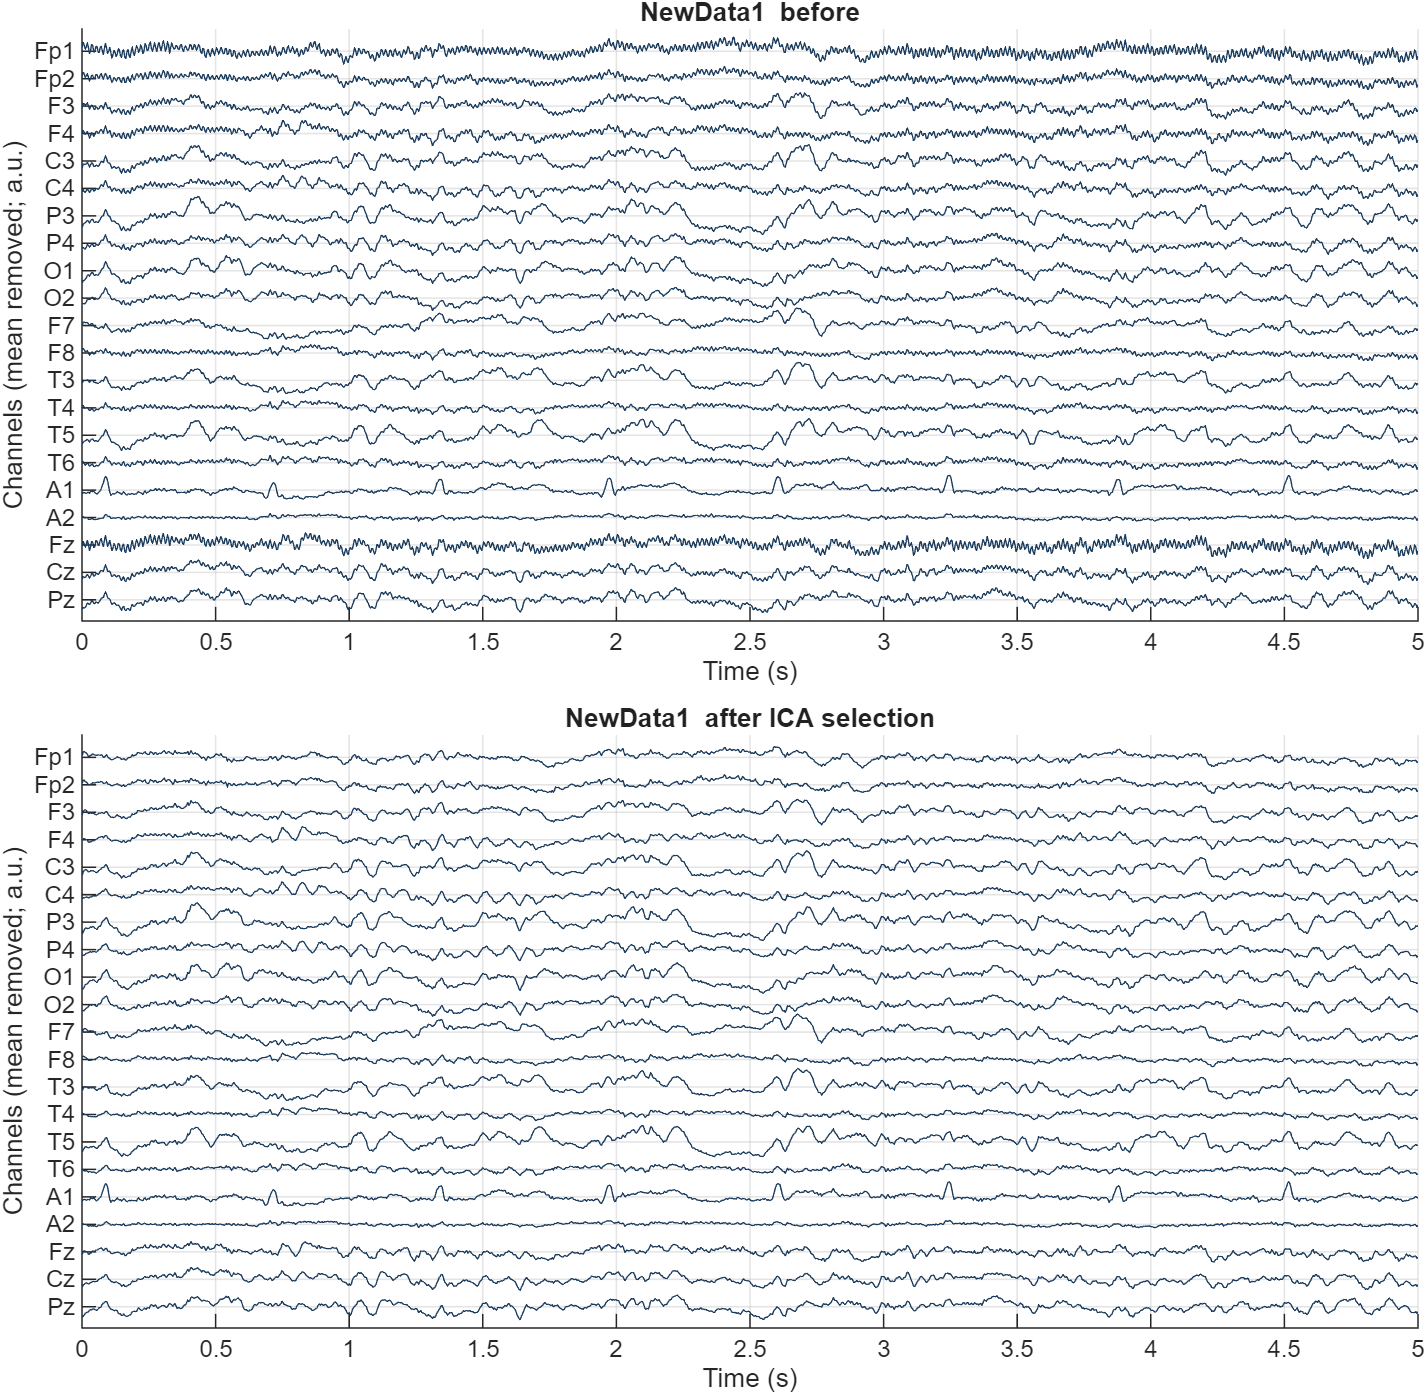
\includegraphics[width=0.85\textwidth,height=0.72\textheight,keepaspectratio]{fig10_newdata1_before_after.png}
\caption{All channels of NewData1 before and after removing IC4; the display is mean-removed and the scale of the two panels is common.}
\label{fig:nd1}
\end{figure}

\subsection*{Selection of components in NewData1}
\subsection*{Questions 3 and 4: Separation and examination of each component}
\begin{taskbox}
\textbf{3.} Apply an ICA algorithm to the signal and obtain the independent components and the mixing matrix. You can use the function \texttt{R2COM.m} (the R2Com algorithm).\\
\textbf{4.} Plot the temporal, spectral and spatial characteristic of each component and decide whether it is desirable or undesirable. To plot the spectral and spatial characteristics you can use \texttt{pwelch.m} (the MATLAB function) and \texttt{plottopomap.m}, respectively. Note: for the temporal and spectral characteristics use the rows of the source matrix, and for the spatial characteristic consider the corresponding columns of the mixing matrix.
\end{taskbox}

COM2R was run with rank 21; $A$ and $W$ have size $21\times21$ and $S$ has size $21\times1251$. For each component, the time series and the PSD were drawn from the corresponding row of $S$, and the spatial map from the corresponding column of $A$. The sheets of all 21 components are given in Figures~26 to~28, and the table of decisions in Appendix~B. Using the column of $W$ instead of the column of $A$ to interpret the sensor propagation pattern is not correct.

IC4 was removed because of the coincidence of three pieces of evidence: a continuous oscillation, a narrow 60~Hz peak and a fixed mixing pattern. In contrast, IC7 has almost periodic events and an appearance similar to cardiac contamination, but it was not removed, because of the absence of an ECG reference and the possibility of ambiguous interpretation in epileptic EEG. Keeping it does not prove that it is brain activity or that it is clean; it is merely a conservative decision.

\subsection*{Question 5: Recording the desired sources and the reconstruction}
\begin{taskbox}
Store the indices of all desired sources in a vector \texttt{SelSources} and reconstruct the denoised signal: $X_{\mathrm{denoised}}=A(:,\mathrm{SelSources})\times S(\mathrm{SelSources},:)$.
\end{taskbox}

\begin{lstlisting}[language=Matlab]
RejectedSources = 4;
SelSources = [1 2 3 5 6 7 8 9 10 11 12 13 14 15 16 17 18 19 20 21];
X_den = A(:,SelSources)*S(SelSources,:) + channelMean;
\end{lstlisting}

By removing one component, the contribution of the remaining 20 components was returned to the sensor space. The ICA method is suitable for this pattern, because the interference has a distinct time course and an approximately constant spatial pattern. This result is not a claim of removing all types of artifacts of this recording.

\subsection*{Question 6: Evaluation before and after}
\begin{taskbox}
Plot the denoised signal and compare it with the original signal. Did you select the correct sources? Was the noise removal performed well? Should step (5) be repeated more carefully?
\end{taskbox}

\begin{equation}
r=\frac{\|X-X_{\mathrm{den}}\|_F^{2}}{\|X-\mu\mathbf{1}^{T}\|_F^{2}}
\end{equation}

\begin{center}
\small
\begin{tabularx}{\textwidth}{@{}>{\raggedright\arraybackslash}Xc>{\raggedright\arraybackslash}X@{}}
\toprule
\textbf{Index} & \textbf{Result} & \textbf{Interpretation}\\
\midrule
Energy ratio of the removed contribution & 0.080883 & The removed share relative to the mean-removed input energy\\
Reduction of the 30--100~Hz power & 5.7978 dB & Attenuation of the high-frequency activity\\
Reduction of the 0.5--4~Hz power & $-0.01986$ dB & A very small and slightly increasing change\\
Median channel correlation & 0.963993 & Relative similarity before and after; there is no clean reference\\
\bottomrule
\end{tabularx}
\end{center}

The energy ratio 0.080883 is not equivalent to ``8.09 percent of the total noise''; it describes the share of the one removed component. Likewise, a high correlation does not prove the validity of the reconstruction relative to a clean EEG. The very small increase in the low-band power is consistent with the fact that the cross-term of the sources in the sensor space is not necessarily non-negative, and it is not necessarily a computational error.

\paragraph{Time and spectral comparison of NewData1.}

\begin{figure}[H]
\centering
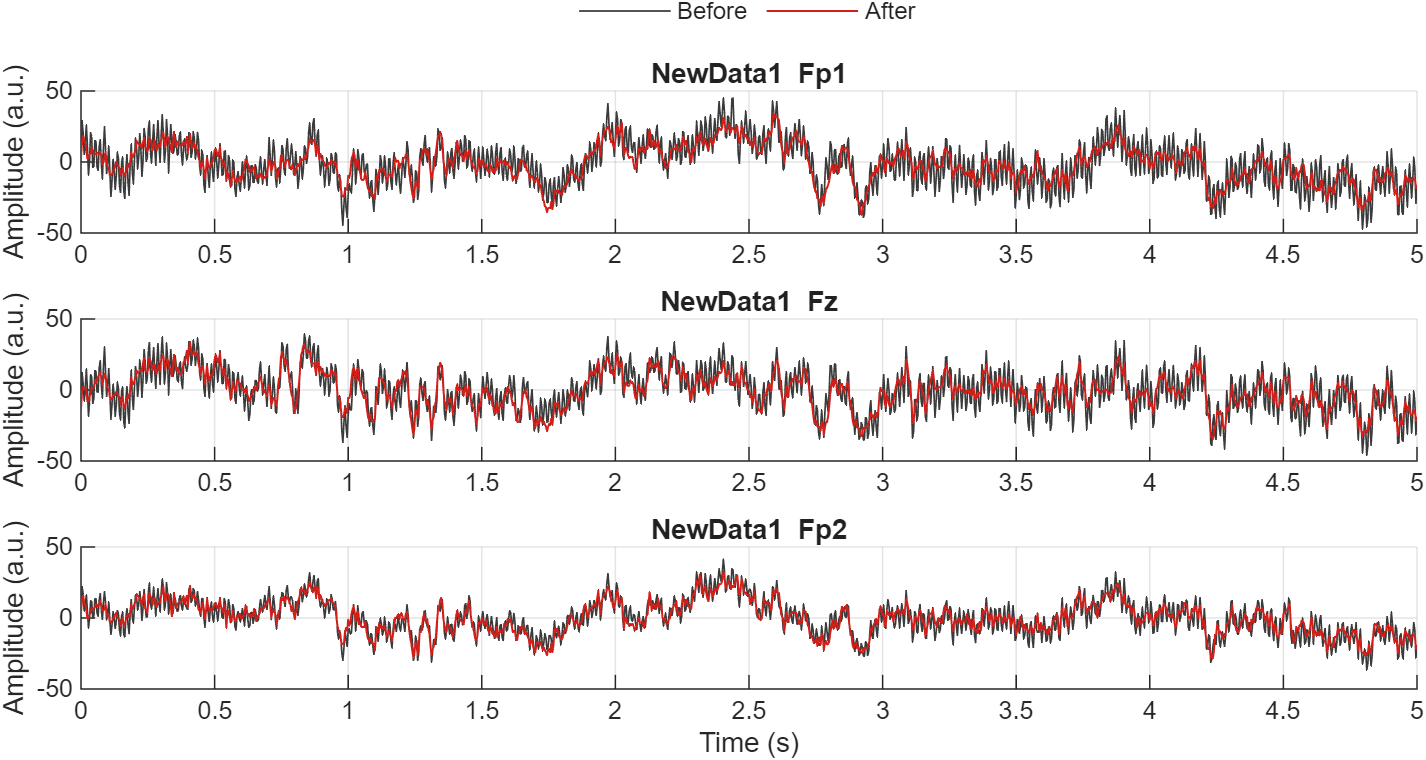
\includegraphics[width=0.9\textwidth]{fig11_newdata1_top_channels.png}
\caption{The channels with the largest RMS of the removed contribution; the fast oscillation is attenuated, but other structures remain.}
\label{fig:nd1top}
\end{figure}

\begin{figure}[H]
\centering
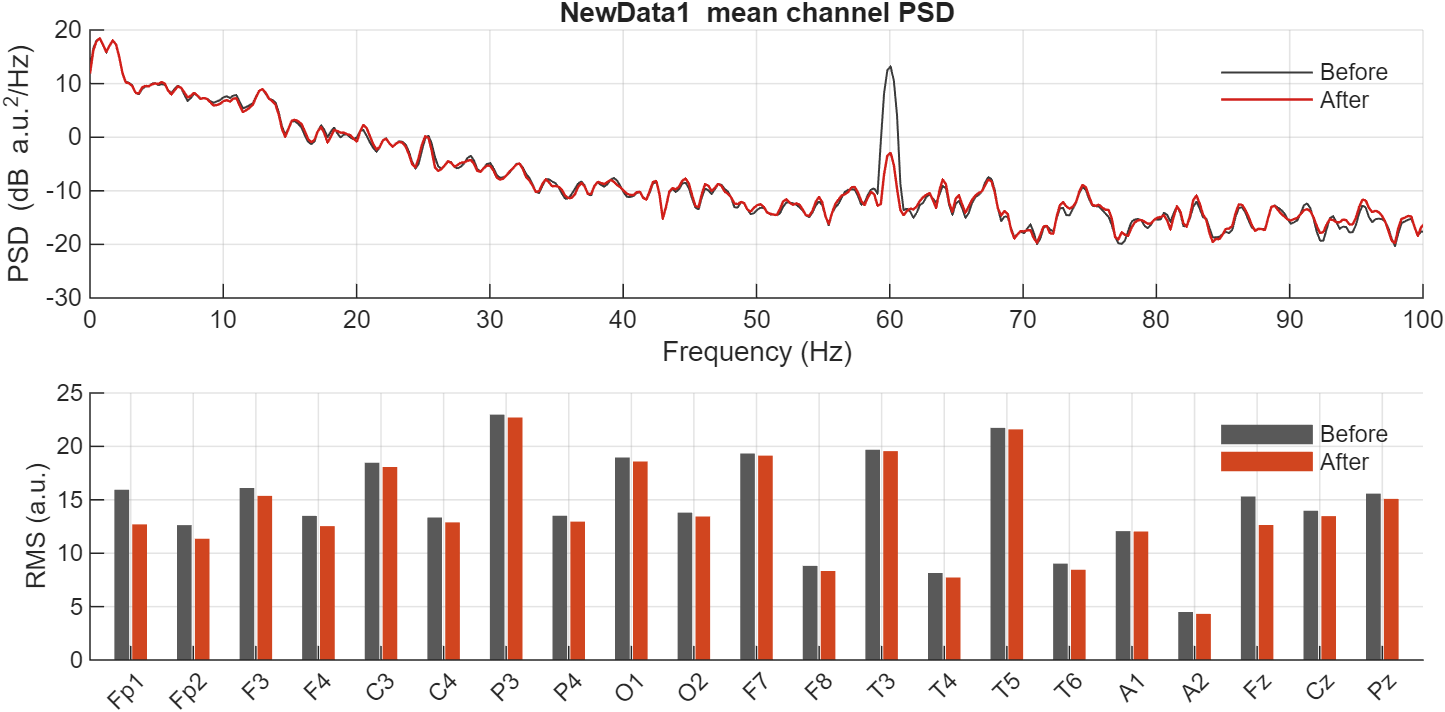
\includegraphics[width=0.9\textwidth]{fig12_newdata1_psd_rms.png}
\caption{Mean PSD and RMS of each channel in NewData1 before and after the removal; a decrease in power does not mean reconstruction accuracy.}
\label{fig:nd1psd}
\end{figure}

The reduction of the peak near 60~Hz, together with the preservation of the major part of the temporal structure, supports the choice of IC4. However, the lack of a clean reference and the retention of IC7 do not allow a claim of complete cleaning. A later review is better carried out with an ECG reference channel or a longer recording, not by the automatic removal of more components.
